% ==================================================
% Rebase Merge 
% Author: Lester James V. Miranda
% ==================================================

\documentclass[preview, convert={outfile=\jobname-out.png,density=300}]{standalone}

\usepackage{tikz}
\usepackage{color}
\usepackage{subfig}
\usepackage{ifthen}

\renewcommand\familydefault{\sfdefault}

\usetikzlibrary{
    matrix,
    shapes,
    fit,
    arrows.meta,
    arrows,
    positioning,
    calc,
    backgrounds,
    shadows.blur,
    shapes.geometric,
}

\begin{document}
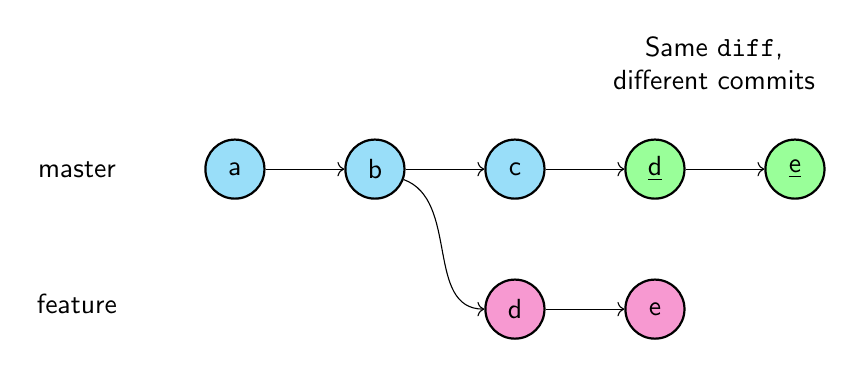
\begin{tikzpicture}[
    node distance= 1cm,
    commit/.style={draw, thick, circle, minimum size=0.75cm},
    master/.style={commit, fill=cyan!40},
    feature/.style={commit, fill=magenta!40},
    textbox/.style={fill=white, align=center, minimum height=0.7cm, minimum width=0.7cm},
]

\node[master] (a) at (0,0) {a};
\node[master] (b) [right=of a] {b};
\node[master] (c) [right=of b] {c};
\node[textbox] (text1) [left=of a] {master};

\node[commit, fill=green!40] (d-new) [right=of c] {\underline{d}};
\node[commit, fill=green!40] (e-new) [right=of d-new] {\underline{e}};

\node[feature] (d) [below=of c] {d};
\node[feature] (e) [right=of d] {e};
\node[textbox] (text2) [below=of text1] {feature};

\draw[->] (a) -- (b) {};
\draw[->] (b) -- (c) {};
\draw[->] (b) to[out=-20, in=180] (d.west) {};
\draw[->] (d) -- (e) {};
\draw[->] (c) -- (d-new) {};
\draw[->] (d-new) -- (e-new) {};

\node[textbox, align=center] (text2) [above=of d-new, xshift=0.75cm, yshift=-0.5cm] {Same \texttt{diff},\\ different commits};

\end{tikzpicture}
\end{document}


